\documentclass[presentation]{beamer}

\usecolortheme{Imperial}
 
\usepackage[utf8]{inputenc}
\usepackage[UKenglish]{babel}
\usepackage{booktabs}
\usepackage{caption}
\usepackage{graphicx}
\usepackage{amsmath}
\usepackage{amsfonts}
\usepackage{amssymb}
\usepackage{epstopdf}
\usepackage{subfigure}
\usepackage{natbib}
\usepackage{bibentry}
\usepackage{listings}
% complying UK date format, i.e. 1 January 2001
\usepackage{datetime}
\let\dateUKenglish\relax
\newdateformat{dateUKenglish}{\THEDAY~\monthname[\THEMONTH] \THEYEAR}

% Imperial College Logo, not to be changed!
\institute{
\includegraphics[height=0.7cm]{Imperial_1_Pantone_solid.eps}

\includegraphics[height=0.7cm]{firedrake-small.pdf}}

% -----------------------------------------------------------------------------




%Information to be included in the title page:
\title{\Large The Firedrake Project: An Introduction}



\author{\small Firedrakers in the workshop:\\ 
Jack Betteridge, Joscha Fregin,\\
Sophia Vorderwuelbecke, Connor Ward}
%{\tiny Imperial College London, Mathematics Departement, Firedrake Research Group\vspace{-1cm}}}
\date{\today}


\setbeamertemplate{navigation symbols}{
    \usebeamerfont{footline}
    \textcolor{blue}{\insertframenumber/\inserttotalframenumber}
}
\usepackage{amsbsy}

\begin{document}

\begin{frame}
    \titlepage
\end{frame}

\begin{frame}{Firedrake \& Finite Element Methods (FEM)}
\begin{itemize}
    \item Automatic code generation
    \item FEM for discretisation of partial differential equations (PDEs)
    \item Encapsulation of different researchers expertise
    \item Increase software productivity
\end{itemize}
\hspace{-0.9cm}
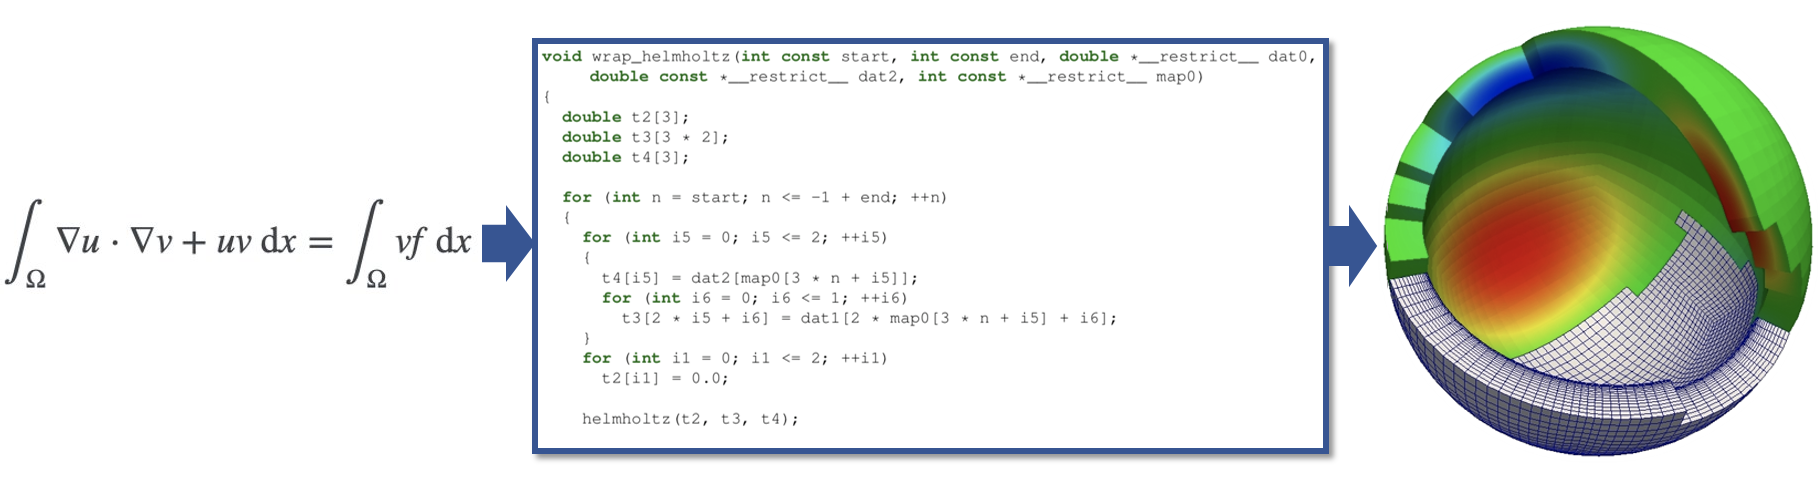
\includegraphics[scale=0.39]{figures/femtopic6.png}

{\tiny Right hand side picture extracted from webpage of Eike Mueller: http://people.bath.ac.uk/em459/research.html}
\end{frame}

\begin{frame}{Example 1: Ice sheet modelling}
\centering

\vspace{0.1cm}
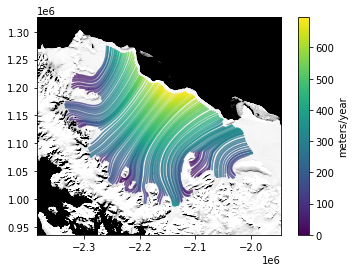
\includegraphics[width=0.8\textwidth]{figures/icepack_demo.png}

{\tiny Shapero, D. et al.: icepack: a new glacier flow modeling package in Python, version 1.0, \\
\vspace{-\baselineskip}Geosci. Model Dev. Discuss. [preprint], in review, 2021}
\end{frame}

\begin{frame}{Example 2: Coastal Ocean Modelling}
\centering
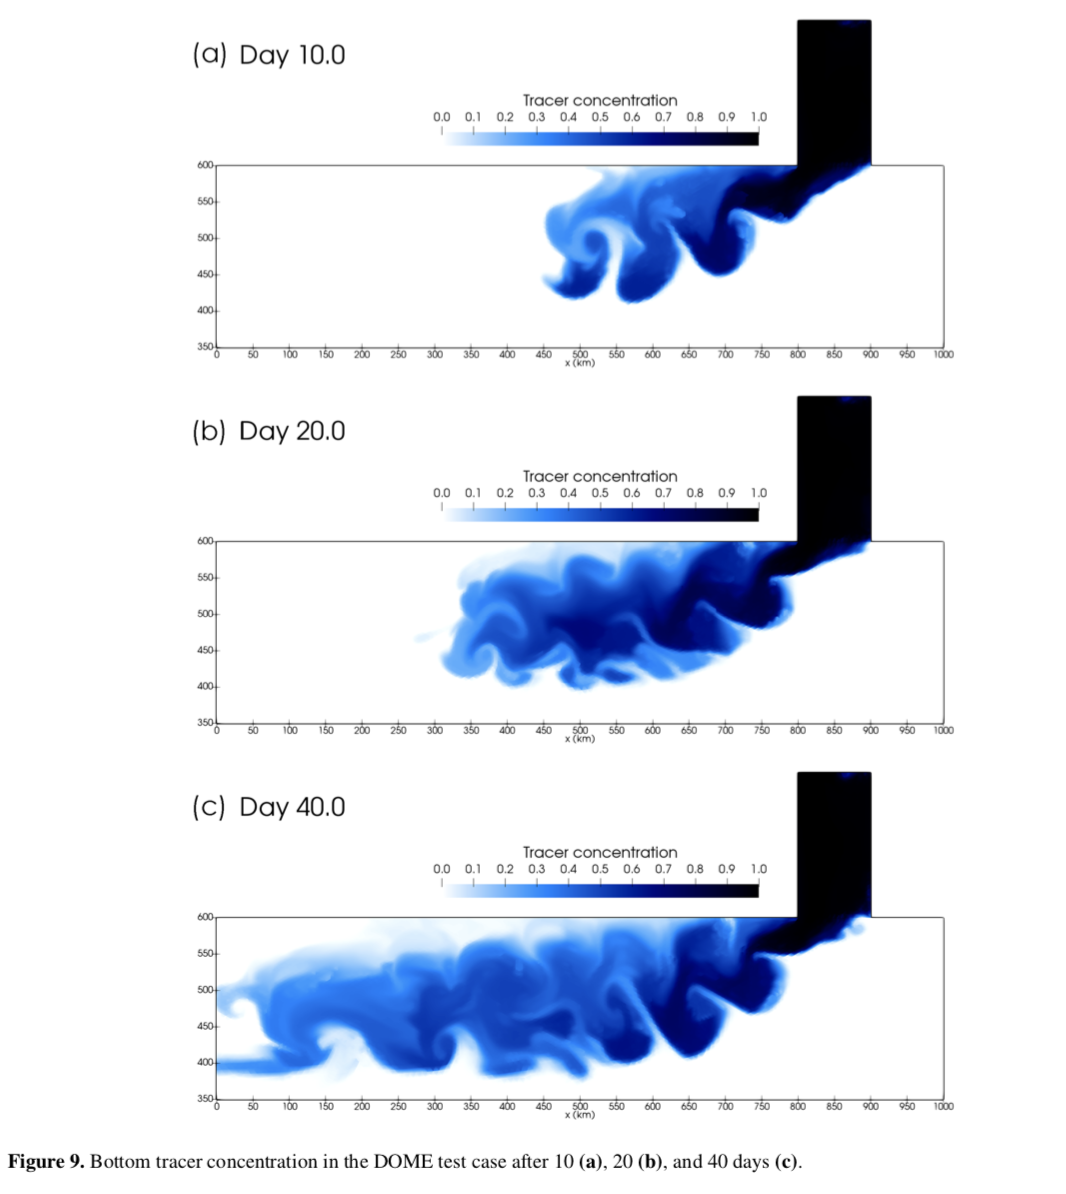
\includegraphics[width=0.5\textwidth]{figures/plume.png}

% icepack: glacier flow modelling
% stream plot of velocity of the antarctic icesheet

\vspace{0.3cm}
{\tiny Kärnä, T. et al.: Thetis coastal ocean model: discontinuous Galerkin discretization\\
\vspace{-\baselineskip}for the three-dimensional hydrostatic equations, Geosci. Model Dev., 11, 4359–4382, 2018}
\end{frame}

% Thetis: coastal ocean modelling
% density-driven overflows
% inflow into stably stratified basin
% forms a coastal plume
% which becomes unstable which results into a generation of eddies and internal waves. 

\begin{frame}{Parallel Algorithms and Libraries}
    \begin{itemize}
        \item Written in Python, compiled to C
        \item PyOP2: global matrix assembly algorithm (and other global operations), explicit distributed memory parallelism with help of MPI (GPUs are WIP)
        \item COFFEE/Loo.py: data level parallelism exploited through vectorisation of local assembly kernels
        \item PETSc: parallel equation system solvers
    \end{itemize}
\end{frame}

\end{document}

